\documentclass{article}
\usepackage[toc,page]{appendix}
\usepackage{blindtext}
\usepackage{titlesec}
\usepackage{graphicx} % Required for inserting images
\usepackage{float}
\usepackage[ddmmyyyy,hhmmss]{datetime}
\usepackage{listings}% http://ctan.org/pkg/listings
\usepackage{amsmath}
\usepackage{hyperref}
\usepackage{biblatex}
\usepackage[dvipsnames]{xcolor}
\usepackage{parskip}
\usepackage[most]{tcolorbox}
\usepackage{lineno}
\linenumbers


\colorlet{myfigurecolor}{teal!90!blue}
\colorlet{myfigurecolorback}{myfigurecolor!10!white}
\colorlet{myexamplecolor}{cyan!40!green}
\colorlet{myexamplecolorback}{myexamplecolor!10!white}
\colorlet{myinlinecolorback}{gray!10!white}
\tcbset{
    enhanced,
    colback=myfigurecolor!5!white,
    boxrule=0.1pt,
    colframe=myfigurecolor,
    fonttitle=\small\bfseries,
    fontupper=\small,
    center title
}

\newtcolorbox[blend into=figures]{myfigure}[2]{
    colback=myfigurecolorback, 
    colframe=myfigurecolor, 
    title={#1},
    label={#2},
    center,
    fontupper=\footnotesize
}

\newtcolorbox[auto counter]{example}[2]{
    colback=myexamplecolorback, 
    colframe=myexamplecolor, 
    title=Example \thetcbcounter: #1, 
    label={#2},
    center,
    breakable,
    fontupper=\footnotesize
}

\addbibresource{references/ref.bib}

\hypersetup{
    colorlinks=true,
    linkcolor=cyan,
    citecolor=cyan,
    filecolor=magenta,      
    urlcolor=cyan,
    pdftitle={Overleaf Example},
    pdfpagemode=FullScreen
}

\definecolor{codegreen}{rgb}{0,0.6,0}
\definecolor{codegray}{rgb}{0.5,0.5,0.5}
\definecolor{codepurple}{rgb}{0.58,0,0.82}
\definecolor{backcolour}{rgb}{0.95,0.95,0.92}

\lstdefinelanguage{elm}
{
  % List of keywords
  morekeywords={
    alias,
    as,
    case,
    else,
    exposing,
    if,
    import,
    in,
    let,
    module,
    of,
    port,
    then,
    type,
    where
  },
  sensitive=true, % Keywords are case-sensitive
  morecomment=[s]{\{-}{-\}}, % s is for start and end delimiter
  morecomment=[l]{--},
  morestring=[b]" % Defines that strings are enclosed in double quotes
}


\lstdefinestyle{inline}{
    basicstyle=\small\ttfamily, % Global Code Style
    captionpos=b, % Position of the Caption (t for top, b for bottom)
    extendedchars=true, % Allows 256 instead of 128 ASCII characters
    tabsize=2, % Number of spaces indented when discovering a tab 
    columns=fixed, % Make all characters equal width
    keepspaces=true, % Does not ignore spaces to fit width, convert tabs to spaces
    breaklines=true, % Wrap lines if they don't fit
    showstringspaces=false, % Lets spaces in strings appear as real spaces
    mathescape=true, % Enable math escape
    commentstyle=\color{codegreen},
    keywordstyle=\color{magenta},
    numberstyle=\tiny\color{codegray},
    stringstyle=\color{codepurple},
    backgroundcolor=\color{myinlinecolorback},   
}

\definecolor{elm-orange}{RGB}{240,173,0}
\definecolor{elm-gray}{RGB}{149,149,138}
\definecolor{elm-blue}{RGB}{0,168,198}

\lstdefinestyle{mystyle}{
    backgroundcolor=\color{myexamplecolorback},   
    commentstyle=\color{codegreen},
    keywordstyle=\color{magenta},
    numberstyle=\tiny\color{codegray},
    stringstyle=\color{codepurple},
    basicstyle=\ttfamily\footnotesize,
    breakatwhitespace=false,         
    breaklines=true,                 
    captionpos=b,                    
    keepspaces=true,                 
    numbers=left,                    
    numbersep=5pt,                  
    showspaces=false,                
    showstringspaces=false,
    showtabs=false,                  
    tabsize=2
}

\newcommand{\mybox}[3]{\begin{center}
\begin{myfigure}{#1}{#2}
\begin{varwidth}{\textwidth}#3\end{varwidth}
\end{myfigure}
\end{center}}

\usepackage{amssymb,graphicx}

\newcommand{\cleftsemicirc}{\put(3.5,2.5){\oval(5,10)[l]}\put(3.5,-2.5){\line(0,0){10}}\phantom{\circ}}
\newcommand{\crightsemicirc}{\put(1.5,2.5){\oval(5,10)[r]}\put(1.5,-2.5){\line(0,0){10}}\phantom{\circ}}
\newcommand{\hole}{\cleftsemicirc \crightsemicirc}
\newcommand{\enc}[1]{\llbracket #1 \rrbracket}
\newcommand{\conf}[2]{\langle #1,#2 \rangle}

\lstset{style=mystyle}

\setlength{\parindent}{0pt} % No indentation
\title{Implementation}
\date{\today}
\author{Sune Skaanning Engtorp}

\begin{document}
\maketitle

\section{Representing syntax}

The generalized editor calculus\cite{aalborg} assumes that it is given an abstract syntax that is represented by a set of sorts $\mathcal{S}$, an arity-indexed family of operators $\mathcal{O}$, and a sort-indexed family of variables $\mathcal{X}$, as per Robert Harper's notation \cite{harper}.

A criterion for the good solution of this project is also the implementation of being able to pretty-print a program into a concrete syntax. For this, it is also necessary for the user to provide the concrete for a language they wish to edit.

It can be a challenge from the user's perspective to provide a specification based on what the calculus assumes. Therefore, it is ideal for the implementation to provide other means of describing the syntax of a language.

In terms of early examples, Metal\cite{metal} has been used in the Mentor \cite{mentor-applications} and CENTAUR \cite{centaur} systems. 
Metal compiles a specification containing concrete syntax, abstract syntax and tree building functions for a formalism $F$ into a Virtual Tree Processor (VTP) formalism, a concrete syntax parser produced by YACC\cite{yacc} and a tree generator which uses VTP primitives to construct abstract syntax trees.

Another example with the same purpose is Zephyr ASDL (Abstract Syntax Description Language)\cite{zephyr}, where the authors have built a tool that converts an ASDL specification into C, C++, Java and ML data-structure definitions. The authors consider ASDL a simpler alternative to other abstract syntax description languages, such as ASN.1 \cite{asn1}.

However, both examples have lack of binding mechanisms in abstract syntax in common. This motivates another possibility of defining a specification language for the to-be-implemented generalized editor itself, which can assist the user in describing the syntax. This would also require a parser that can parse the necessary information assumed by the calculus (including binders). Picking this route allows the project to avoid spending time analyzing different tools and developing a workaround for binders.

\subsection{Specification language}

The specification language is chosen to expect some syntactic categories followed by concrete and abstract syntax in BNF notation.  %Every operator from the abstract syntax is represented by one or more non-terminals in the concrete syntax.
Every syntactic category is represented by one or more non-terminals with a term, arity and operator name. The term might refer to other syntactic categories or its own. Each term is the concrete syntax of an operator, while the arity, in combination with the operator name, is a concise representation of the abstract syntax of an operator. 
The abstract syntax only makes use of the defined syntactic categories and, inspired by Harper\cite{harper}, binders can be specified in the arity description with a dot ('.'), e.g. $x.s$ specifies that variable $x$ is bound within the scope of $s$.

% The specification language itself can be described with BNF notation (with some informal notation for newlines and strings), as seen in figure \ref{fig:spec-lang-bnf}.

% \begin{myfigure}{Description of the specification language itself}{spec-lang-bnf}
% \[
% \begin{aligned}
% syntax                  &::= \textit{category-list} \ \text{<new-line>} \ \textit{rule-list} \ \text{<new-line>} \ \textit{crule-list}  &&\\
% category                &::= term \ `\in\textrm' \ term \ | \ \epsilon &&\\
% \textit{category-list}  &::= category \ | \ \textit{category-list} \ \text{<new-line>} \ category &&\\
% rule                    &::= term \ `::=\textrm' \ exp \ | \ \epsilon &&\\
% \textit{rule-list}      &::= rule \ | \ \textit{rule-list} \ `|\textrm' \ rule &&\\
% crule                    &::= \ `<\textrm'\textit{ term }`>\textrm' \ `::=\textrm' \ exp \ | \ \epsilon &&\\
% \textit{crule-list}      &::= crule \ | \ \textit{crule-list} \ `|\textrm' \ crule &&\\
% exp                     &::= \text{<any-string>} &&\\
% term                    &::= \text{<alpha-numeric-string>}
% \end{aligned}
% \]
% \end{myfigure}

From this specification language, it is possible to extract what is assumed by the generalized editor calculus\cite{aalborg}. The set of sorts $\mathcal{S}$ is the set of syntactic categories. For example, a syntactic category $e \in Exp$ can get parsed into a sort $s_{e}$.
The family of arity-indexed operators $\mathcal{O}$ can be extracted from the BNF notation since each derivation rule represents an operator with a specified arity.

\begin{example}{Syntax of a small C language}{ex:c-spec}
Following is a specification of a subset of the C language\cite{c-iso-standard}, per the described specification language.
\[
\begin{aligned}
&\textit{p}         \in \textit{Prog}           \quad &\textit{s}           \in \textit{Stmt}       \\
&\textit{vd}        \in \textit{VariableDecl}   \quad &\textit{fd}        \in \textit{FunDecl} \\
&\textit{t}         \in \textit{Type}           \quad &\textit{id}          \in \textit{Id}         \\
&\textit{e}         \in \textit{Exp}            \quad &\textit{b}           \in \textit{Block}      \\
&\textit{fa}        \in \textit{Funarg}         \quad &\textit{cond}      \in \textit{Conditional}    \\
&\textit{int}       \in \textit{Int}            \quad &\textit{char}        \in \textit{Char}       \\
&\textit{bool}       \in \textit{Bool}          \quad &\textit{string}        \in \textit{String}       \\
\end{aligned}
\]
\[
\begin{aligned}
&\text{Sort}&   & \text{Term}&                                      &\text{Arity}&                  & \text{Operator}               \\
&p ::=      &   & \textit{fd}&                                      &(fd)p       &                  &program                \\
&b ::=      &   & \text{$bi$}&                                      &(bi)b       &                  &block                \\
&bi ::=      &   &\text{$vd$}&                                      &(vd)bi       &                 &blockdecls                \\
&\quad |     &  & \text{$s$}&                                       &(s)bi       &                  &blockstmts                \\
&\quad |    &   & \epsilon &                                        &()bi          &                &blockdone              \\
&vd ::=      &  & \text{$t$ $id$ "=" $e$ ";" $bi$}&                 &(t,e,id.bi)s &                 &vardecl                \\               
&\textit{fd} ::=&& \text{$t_1$ $id_1$ "(" $t_2$ $id_2$ ")"}&        &(t_1,id_1.fd,&                 &\textit{fundecl1}      \\                
&           &   & \text{"\{" $b$ "\}" \textit{fd}}&                 &t_2,id_2.b)fd\\
&\quad |    &   & \text{$t_1$ $id_1$ "(" $t_2$ $id_2$ ","}&         &(t_1,id_1.fd,t_2, &            &\textit{fundecl2}\\
&           &   & \text{$t_3$ $id_3$ ") \{" $b$ "\}" $\textit{fd}$}& &t_3,id_2.id_3.b)\textit{fd}\\
&\quad |    &   & \text{$\epsilon$}&                                &()fd &                         &\textit{fundecldone}             \\
&s ::=      &   & \text{$id$ "=" $e$ ";"}&                          &(id,e)s &                      &assignment             \\
&\quad |    &   & \text{$id$ "(" \textit{fa} ");"}&                 &(id,\textit{fa})s&             &\textit{stmtfuncall}             \\
&\quad |    &   & \text{"return " $e$ ";"}&                         &(e)s        &                  &return             \\
&\quad |    &   & \text{$cond$}&                                    &(cond)s        &               &conditional             \\
&\quad |    &   & \text{$s$ $s$}&                                   &(s,s)s        &                &compstmt             \\
&fa ::=     &   & \text{$t$ $id$}&                                  &(t,id)\textit{fa} &            &\textit{funarg}                \\
&\quad |    &   & \text{$t$ $id$ "," $fa$}&                         &(t,id,\textit{fa})\textit{fa} &&\textit{funargs}                \\
&cond ::=   &   & \text{"if (" $e$ ") \{" $b_1$ "\} else \{" $b_2$ "\}"}&&(e,b_1,b_2)cond &         &\textit{ifelse}             \\
&t ::=      &   & "int"&                                            &()t        &                   &tint               \\
&\quad |    &   & "char"&                                           &()t        &                   &tchar              \\
&\quad |    &   & "bool"&                                           &()t        &                   &tbool              \\
&e ::=      &   & int&                                              &(int)e        &                &int                \\
&\quad |    &   & char&                                             &(char)e        &               &char               \\
&\quad |    &   & bool&                                             &(bool)e        &               &bool               \\
&\quad |    &   & \text{$e_1$ "+" $e_2$}               &            &(e_1,e_2)e  &                  &plus               \\
&\quad |    &   & \text{$e_1$ "==" $e_2$}               &           &(e_1,e_2)e  &                  &equals               \\
&\quad |    &   & \text{$id$ "(" \textit{fa} ")"}&                  &(id,\textit{fa})e&             &\textit{expfuncall}             \\
&\quad |    &   & \text{$id$}&                                      &(id)e&                         &expident             \\
&id ::=     &   & \%\text{string}&                                  &()id        &                  &ident              \\
\end{aligned}
\]
'\%int', '\%char', '\%string' and '\%bool' are meta-variables representing any parseable integer, character, sequence of characters and boolean constant by the C language.

This subset is chosen as it can represent a C program consisting of only function declarations at the top level, where one of them might represent a \texttt{main} function, the entry point of a C program. The identifier of a function declaration is bound within the following function declarations (e.g. $id_1$ is bound within $\textit{fd}$ in the $\textit{fundecl1}$ operator).

A limitation of this specification is recursive function calls. Ideally, the identifier in a function declaration is bound both within the function block and the sequence of following function declarations. However, this would result in the same identifier appearing twice in the arity definition. E.g. the arity for the $\textit{fundecl1}$ operator is $(t_1,id_1.\textit{fd},t_2,id_2.b)fd$ where $id_1$ is the identifier of the function, which ideally would be bound in both \textit{fd} (the following sequence of function declarations) and $b$ (the function block). 

Another limitation, or something that might seem unnecessary, is having the $blockdone$ and $fundecldone$ operators. They are necessary to allow for a block to end with a $vardecl$ operator and to end a sequence of function declarations with the $fundecl1$ or $fundecl2$ operator. This a pattern that allows operators to bind identifiers within the following terms.

\end{example}
\begin{example}{Syntax of a small SQL language}{ex:as-sql-lang}
Below is the syntax of a subset of the PostgreSQL\cite{postgresql-about} dialect of SQL:
\[
\begin{aligned}
&\textit{q} \in \textit{Query}          \\
&\textit{cmd} \in \textit{Command}      \quad &\textit{id} \in \textit{Id} \\
&\textit{const} \in \textit{Const}      \quad &\textit{clause} \in \textit{Clause} \\
&\textit{cond} \in \textit{Condition}   \quad &\textit{exp} \in \textit{Expression} \\
\end{aligned}
\]
\\
\[
\begin{aligned}
&\text{Sort}&   &\text{Term}&                                       &\text{Arity}&              &\text{Operator}            \\
&query ::=&     &\text{"SELECT " $id_1$}&                           &(id_1,id_2,clause)query&   &select                       \\
&           &   &\text{" FROM " $id_2$ $clause$}\\
& cmd ::=&      &\text{"INSERT INTO " $id_1$}&                      &(id_1,id_2.query)cmd&      &insert                   \\
&           &   &\text{" AS " $id_2$ $query$}&\\
&id ::=&        &\text{\%string}&                                   &()id&                      &id                   \\
&const ::=&     &\text{\%number}&                                   &()const&                   &num                   \\
& \quad | &     &\text{"'"\%string"'"}&                             &()const&                   &str                \\
&clause ::=&    &\text{"WHERE " $cond$}&                            &(cond)clause&              &where                   \\
& \quad | &     &\text{"HAVING " $cond$}&                           &(cond)clause&              &having                \\
&cond ::=&      &\text{$exp_1$ ">" $exp_2$}&                        &(exp_1,exp_2)cond&         &greater                   \\
& \quad | &     &\text{$exp_1$ "=" $exp_2$}&                        &(exp_1,exp_2)cond&         &equals                \\
&exp ::=&       &\text{$const$}&                                    &()exp&                     &econst                   \\
& \quad | &     &\text{$id$}&                                       &()exp&                     &eid                \\
\end{aligned}
\]
where '\%string' and '\%number' and '\%char' are placeholders for any parsable sequence of characters and numbers by the PostgreSQL language.

This subset is chosen as it can represent simple select queries and insert commands.

Notably, a binder is used in the $insert$ operator, where the alias of $id_1$, specified as $id_2$ is bound within the sub-query.
\end{example}

To make the specification language parseable, a more computer-friendly format is presented in figure \ref{fig:spec-lang-bnf}. Every syntactic category is expected on its own line, followed by a blank line and all derivations. Each derivation is expected to be a syntactic category, followed by '::=' and every term (which acts as the concrete syntax of an operator), arity and operator name, separated with a vertical bar '|'. Every term, arity and operator are separated with a number-sign '\#'. See figure \ref{fig:sql-lang-parseable} for an example.

\begin{myfigure}{Specification language in BNF notation}{fig:spec-lang-bnf}

\end{myfigure}

\begin{myfigure}{Subset of syntax of a small SQL language in a parseable format}{fig:sql-lang-parseable}
\begin{lstlisting}
query in Query
cmd in Command
id in Id
clause in Clause

query ::= " SELECT " id " FROM " id clause # (id,id,clause)query # select
cmd ::= " INSERT INTO " id " AS " id query # (id,id.query)cmd # insert
\end{lstlisting}

It is also assumed that the first non-terminal from the derivations is the starting symbol.

\end{myfigure}

\section{Specialization and parameterization}
Neil D. Jones has presented the notion of partial evaluation in terms of program specialization\cite{jones96}, where a partial evaluator receives a general program and some static input, which results in a specialized program that, if specialized in a meaningful way, performs better than the original program. An example provided by Jones is a program computing $x^n$ (program $p$ in listing \ref{lst:jones-ex1}), which can be specialized to having $n = 5$ (program $p_5$ in listing \ref{lst:jones-ex2}), unfolding the recursive calls and reducing $x*1$ to $x$. Formally, the general program $p$ and static input $in_1$ is passed to a partial evaluator $mix$, which outputs a specialized program $p_{in_1}$, which can take dynamic input $in_2$ and produce some output.

\begin{lstlisting}[style=inline,label={lst:jones-ex1},caption={Two-input program $p$}]
f(n, x) = if n = 0 then 1
else if even(n) then f (n/2,x)^2
else x * f(n-1,x)
\end{lstlisting}

\begin{lstlisting}[style=inline,label={lst:jones-ex2},caption={Specialization of program $p$}]
f5(x) = x * ((x^2)^2)
\end{lstlisting}

This idea of specialization can also be applied to this project's implementation, where the static input is the syntax of a language, which if partially evaluated with a general program, results in a specialized program. This program represents a syntax-directed editor instance for the static input's language, which can take dynamic input in the form of editor expressions, resulting in either cursor movement or updates to the target language's program.

In other words, an editor can be specialized given some syntax, potentially skipping the process of parsing syntax and generating source code every time a user wishes to use the same editor instance for some language. Not only does this provide better performance, but it forces a modular design and a parameterization strategy which ensures that only relevant parts of the program considers a given syntax.

The overall implementation strategy will be influenced from the informal overview of necessary steps to instantiate an editor based on a language's specification (\ref{fig:overview-steps}).

\begin{myfigure}{Informal overview of steps to instantiate an editor}{fig:overview-steps}
\begin{enumerate}
    \item Extract a set of sorts $\mathcal{S}$ and an arity-indexed family of operators $\mathcal{O}$ from the specification
    \item For every sort $s \in \mathcal{S}$, add a $hole_s$ operator with arity $()s$ and a $cursor_s$ operator with arity $(s)s$ to $\mathcal{O}$, as per definition \ref{X}
    \item Create the sorts and family of cursorless operators, as per definition \ref{X}
    \item Create the sorts and family of operators containing a cursor context, as per definition \ref{X}
    \item Create the sorts and family of operators for well-formed trees, as per definition \ref{X}
\end{enumerate}
\end{myfigure}

With the sorts and family of operators, there should be functions supporting every editor expression $E \in Edt$ (figure \ref{x}), which will apply an editor expression on a given well-formed tree containing exactly one cursor.  

Another important thing consideration for the implementation is whether part of the editor's source code should be generated automatically, or if a generic model might suffice.

Automatic generation of source code offers the benefit of directly representing provided operators, along with their arity and sort, within an algebraic data type (referred to as type in Elm and data in Haskell). This ensures that only well-formed terms can be represented using the algebraic data types.

However, opting for this method might require automatic updates to both the definitions and signatures of some functions. This presents a challenge in ensuring that these functions maintain their intended behaviour after the updates.

\begin{example}{Algebraic data types for a small C syntax}{ex:c-alg-data-types}
Given example \ref{ex:c-spec}, one can generate the following custom types in Elm:
\begin{lstlisting}
type alias Bind a b =
    ( a, b )
type Prog
    = Program FunDecls
type Block
    = Block BlockItems
type BlockItems
    = BlockDecl VarDecls
    | BlockStmts Statements
    | BlockDone
type VarDecls
    = VarDecl Type Id Exp BlockItems
type FunDecls
    = FunDecl1 Type (Bind Id FunDecls) Type (Bind Id Block)
    | FunDecl2 Type (Bind Id FunDecls) Type (Bind Id (Bind Id Block))
    | FunDeclDone
type Statement
    = Assignment Id Exp
    | StmtFunCall Id Funargs
    | Return Exp
    | Conditional Conditional
type Funargs
    = ArgSingle Funarg
    | ArgCompound Funargs Funarg
type Funarg
    = Funarg Type Id
type Conditional
    = IfElse Exp Block Block
type Statements
    = SSingle Statement
    | SCompound Statements Statement
type Type
    = TInt
    | TChar
    | TBool
type Exp
    = Num
    | Char
    | Bool
    | Plus Exp Exp
    | Equals Exp Exp
    | ExpFunCall Id Funargs
    | ExpId Id
type Id
    = Ident String
\end{lstlisting}

The $Bind$ type alias is simply a tuple of 2 given type variables. This would be a part of the generated source code. 
\end{example}

In contrast, a generic solution without the need for generating new source reduces the risk of syntax errors in the target language for the editor itself. A generic solution involves designing a model capable of holding the necessary information from any syntax. An approach for this is provided in figure \ref{fig:generic-types}. However, this approach requires additional well-formedness checks on any given term concerning the syntax.

As an alternative to having specific types for each given syntactic category (as in example \ref{ex:c-alg-data-types}), one can design a generic model with records in Elm, as in listing \ref{lst:elm-ex}.

\begin{lstlisting}[backgroundcolor=\color{myfigurecolorback},caption={Elm Records for storing syntax information},label={lst:elm-ex}]
type alias Syntax =
{ synCats : [String]
, operators : [Operator]
}

type alias Operator =
{ name : String
, arity : (Maybe [String], String)
, concSyn : String
}
\end{lstlisting}

The arity in the Operator type is a tuple, where the first entry is a potential list of identifiers bound within the term in the second element of the tuple.  

In Haskell, this corresponds to named fields\cite{haskell-records-named-fields}, which have a very similar syntax.

The implementation will proceed with automatic generation of source code, including algebraic data types, due to their advantage in handling ill-formed terms effectively. If given an ill-formed term, it is considered ill-typed by the editor, which poses an advantage over the generic solution requiring thorough checking to ensure that given terms are well-formed.

\section{Generating source code}
Elm CodeGen\cite{elm-codegen-package} is an Elm package and CLI tool (command-line interface tool) to generate Elm source code. The tool is an alternative to the otherwise obvious (and arguably tedious) strategy of having a source code template, where certain placeholders are replaced with relevant data or code snippets associated with the parsed syntax.

Besides offering the ability to generate source code, it offers offers automatic imports and built-in type inference. Example usage of Elm CodeGen from the documentation\cite{elm-codegen-package} is given in figure \ref{fig:codegen-ex}.

\begin{myfigure}{Elm CodeGen usage}{fig:codegen-ex}
Following declares an Elm record and passes it to a \texttt{ToString} function: 

\begin{lstlisting}[backgroundcolor=\color{myfigurecolorback},language=elm]
Elm.declaration "anExample"
    (Elm.record
        [ ("name", Elm.string "a fancy string!")
        , ("fancy", Elm.bool True)
        ]
    )
    |> Elm.ToString.declaration
\end{lstlisting}

The above will generate following string:
\begin{lstlisting}[backgroundcolor=\color{myfigurecolorback},language=elm]
anExample : { name : String, fancy : Bool }
anExample =
    { name = "a fancy string!"
    , fancy = True
    }
\end{lstlisting}
\end{myfigure}

Using Elm CodeGen offers the advantage of integrating a parser, which, if implemented in Elm as well, can directly produce the data to enable Elm Codegen to produce source files for the editor. 

More specifically, the implementation will use the built-in \texttt{Parser} Elm library to parse a \texttt{RawSyntax} object (see listing \ref{lst:raw-syntax-model}), which is a direct representation of the syntax as specified in the specification language (figure \ref{fig:spec-lang-bnf}). 

\begin{lstlisting}[language=elm,style=inline,caption={Raw syntax model in Elm},label={lst:raw-syntax-model}]
type alias RawSyntax =
    { synCats : List RawSynCat
    , synCatRules : List RawSynCatRules
    }

type alias RawSynCatRules =
    { synCat : String
    , operators : List RawOp
    }

type alias RawOp =
    { term : String
    , arity : String
    , name : String
    }

type alias RawSynCat =
    { exp : String
    , set : String
    }
\end{lstlisting}

If parsing of the raw syntax is successful, the string-representation of the arity will be transformed into its own \texttt{Arity} type (listing \ref{lst:arity-model}), which is a simple list of tuples, where the first element is a list of variables to be bound within the second element.

\begin{lstlisting}[language=elm,style=inline,caption={Arity model},label={lst:arity-model}]
type alias Arity =
    List ( List String, String )
\end{lstlisting}

Further transformations will be made, following the informal implementation steps (figure \ref{fig:overview-steps}), such as adding $hole$ and $cursor$ operators and creating other sets sorts and family of operators. 

Every set of sorts and family of operators are stored in a model very similar to listing \ref{lst:raw-syntax-model}, but where the arity is replaced with an arity of the type provided in listing \ref{lst:arity-model}.

Having all expected sets of sorts and family of operators, i.e. the abstract syntax extended with $hole$ and $cursor$ operator $\mathcal{S}, \mathcal{O}$, cursorless trees $\hat{\mathcal{O}},\hat{\mathcal{S}}$, cursor contexts $\mathcal{S}^C,\mathcal{O}^C$ and well-formed trees $\dot{\mathcal{O}},\dot{\mathcal{S}}$, the CodeGen package can generate algebraic data types for every sort and its operators and separate them into their own separate modules (files). 

\begin{example}{From specification parser to Elm CodeGen for small C-language}{ex:parser-to-elm-codegen}
Given the specification in example \ref{ex:c-spec}, the parser can produce following \texttt{Declaration} for the \texttt{Statement} algebraic data type in example \ref{ex:c-alg-data-types}:
\begin{lstlisting}[backgroundcolor=\color{myexamplecolorback},language=elm]
Elm.customType "Statement"
            [ Elm.variantWith "Assignment" 
                [ Elm.Annotation.named [] "Id", 
                  Elm.Annotation.named [] "Exp" ]
            , Elm.variantWith "StmtFunCall" 
                [ Elm.Annotation.named [] "Id", 
                  Elm.Annotation.named [] "Funargs" ]
            , Elm.variantWith "Return" 
                [ Elm.Annotation.named [] "Exp" ]
            , Elm.variantWith "Conditional" 
                [ Elm.Annotation.named [] "Conditional" ] ]
\end{lstlisting}

This declaration, if passed to Elm CodeGen's \texttt{File} function, would generate a source file with following contents:
\begin{lstlisting}[backgroundcolor=\color{myexamplecolorback},language=elm]
type Statement
    = Assignment Id Exp
    | StmtFunCall Id Funargs
    | Return Exp
    | Conditional Conditional
\end{lstlisting}
\end{example}


% The process of considering this can be alleviated by describing the overall steps necessary for the program to instantiate an editor for a given (abstract and concrete) syntax:

% \begin{enumerate}
%     \item A set of sorts $\mathcal{S}$ and an arity-indexed family of operators $\mathcal{O}$ is extracted from the specifications
%     \item For every sort $s \in \mathcal{S}$, add a $hole_s$ with arity $()s$ and $cursor_s$ operator with arity $(s)s$ to $\mathcal{O}$
%     \item Create cursorless sorts and operators
%     \item Create cursor context sorts and operators
%     \item Create well-formed sorts and operators
%     \item Editor expressions are represented as pre-defined functions that with respect to 
%     \item Cursor movement is also represented as pre-defined functions that with respect to parsed operators will do movement
%     \item Satisfaction rules for modal operators are pre-defined functions that wrt. some parsed operators and an arbitrary abt, it can figure out whether or not a given cursor context is encapsulating some operator
% \end{enumerate}

Having generated all sorts and operators as algebraic data types in Elm, the next step is to implement functionality for editor expressions. For example, consider the cursor substitution operator (definition \ref{X}), where the editor calculus enforces that operators can only be substituted with operators of same sort. Initially, a straightforward approach involves having a substitution function for each sort $s \in \mathcal{S}$. This approach of course leads an implementer to consider generalization, i.e. how a single function can take any cursor-encapsulated abt and replace it with an operator of the same sort. A solution to this could be 
% % TODO: replace this with a more interesting example, i.e. conditionals
using type classes, where we might have a type class called \texttt{substitutable} and either a specific instance for each sort or a generic instance for all sorts. Having a specific instance for each sort also leads to some amount of boilerplate, but serves the advantage of having a single function definition for the actual cursor substitution. This solution might also apply to other editor expressions.
Having a typeclass is possible in Haskell (see listing \ref{lst:haskell-typeclass}), but typeclasses are not directly supported by Elm. They can however be simulated with Elm records, as shown in the "typeclasses" Elm package\cite{elm-typeclass-package}. An example of such a simulation is shown in listing \ref{lst:elm-typeclass}.

% TODO: replace this with a more interesting example, i.e. conditionals
\begin{lstlisting}[language=Haskell,style=inline,caption={Haskell typeclass example},label={lst:haskell-typeclass}]
-- typeclass
class Substitutable a where 
    substitute :: a -> a -> a
    
-- instance of typeclass
instance Substitutable a where
    substitute _ replacement = replacement

-- example usage
doIntSub :: Int
doIntSub = substitute 1 2 
\end{lstlisting}


% TODO: replace this with a more interesting example, i.e. conditionals
\begin{lstlisting}[language=elm,style=inline,caption={Elm typeclass simulation example},label={lst:elm-typeclass}]
{-| Simulate a type class
-}
type alias Substitutable a =
    { substitute : a -> a -> a }

{-| Generic instance of the typeclass, we don't need any specific implementation for each type/sort, we just want to assure that the expression and replacement are of the same type. This is constrained by the `substitute` function signature in the (simulated) typeclass.
-}
substituteAny : Substitutable a
substituteAny =
    { substitute = \_ replacement -> replacement }

{-| Polymorphic function that can be used with any type that has an instance of the `Substitutable` typeclass.
-}
substitute : Substitutable a -> a -> a -> a
substitute substitutable expression replacement =
    substitutable.substitute expression replacement

{-| Example usage
-}
doIntSub : Int
doIntSub =
    substitute substituteAny 1 2
\end{lstlisting}

\section{Decomposing trees}
The implementation needs to be able to check if a given abt is well-formed, or in other words, if it can be interpreted as $C[\dot{a}]$, where $C$ is a cursor-context (definition \ref{def:cursor-context}) and $\dot{a}$ is a well-formed abt (definition \ref{def:well-formed}). 

The generalized editor calculus\cite{aalborg} defines well-formed trees as abt's with exactly one cursor either as the root or as an argument of the root. However this definition, in conjunction with the cursor context definition, leads to multiple valid decompositions for an abt in certain scenarios, which is also mentioned in \cite{aalborg}. This is when the cursor is located at one of the immediate children of the root. In that case, the cursor context can be interpreted as either the tree where the cursor has been replaced with a context hole, or it can be interpreted as an empty context. For example, consider a small tree created from the syntax given in example \ref{ex:as-sql-lang} (including cursor and hole operators) and their two possible decompositions in figure \ref{fig:sql-decomp-ex}.

\begin{figure}[H]
    \centering
    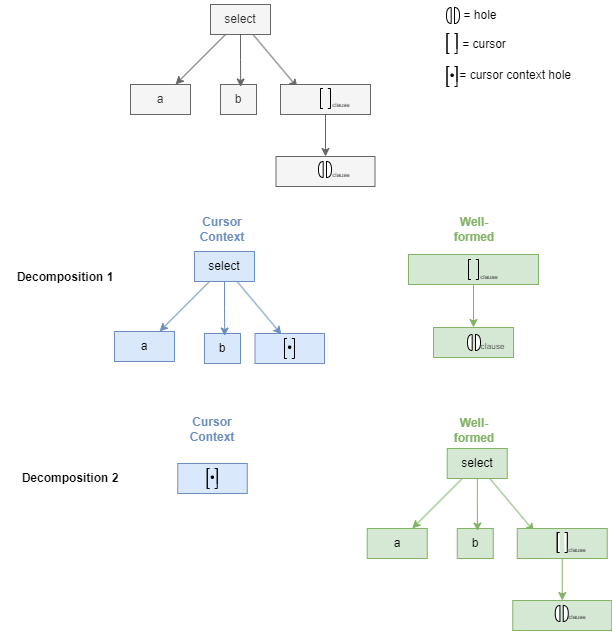
\includegraphics[width=\textwidth]{img/slq-decompose-ex.drawio.png}
    \caption{Two different decompositions of the same term}
    \label{fig:sql-decomp-ex}
\end{figure}

Since decomposition should be possible on any sort of any given syntax, we have a typeclass called \texttt{decomposable} that contains a method called \texttt{decompose} which takes a statement made up by the operators of sort $\mathcal{S}$, and returns a cursor-context and well-formed-tree pair, if decomposition is possible.

In order to instantiate the \texttt{decomposable} type class for any sort, it is then necessary to specify how we for any term in any sort, can decompose uniquely into a cursor context and well-formed-tree pair. 

Decomposition of an abt can be defined algorithmically and divided into following sub-tasks:
\begin{itemize}
    \item Locate the cursor in the tree to be decomposed and generate a path to the cursor
    \item Generate an abt of sort $s^C \in \mathcal{S}^C$ based on the cursor path
    \item Generate an abt of sort $\dot{s} \in \dot{\mathcal{S}}$ based on the rest of the tree that was not traversed when generating the cursor context
\end{itemize}

The following will explain in more details how the steps above can be done, and how we always get a unique decomposition, as long as the abt to be decomposed is well-formed. 

\subsection{Cursor path}

Generating a path to the cursor in the abt of sort $s \in \mathcal{S}$ extended with hole and cursor operators (definition \ref{def:holes-cursors-extension}) simplifies the process of generating the cursor context. The path tells us which operator $o^C \in \mathcal{O}^C$ replaces each $o \in \mathcal{O}$. 
The list can be generated by performing pre-order traversal of the tree to be decomposed, extending the list with every $i$, representing which argument in an operator of arity $(\vec{s}_1.s_1, ... , \vec{s}_i.s_i, ..., \vec{s}_n.s_n)\mathcal{S}$ was followed to locate the cursor.

The implementation of such a function depends on the set of sorts $\mathcal{S}$ and arity-indexed family of operators $\mathcal{O}$ given by the abstract syntax of a language. The Elm CodeGen\cite{elm-codegen-package} 

\subsection{Cursor context}

First, the cursor context is built by performing pre-order traversal the tree to be decomposed, substituting every operator $o \in \mathcal{O}$ for its corresponding cursor context operator $\hat{o} \in \hat{\mathcal{O}}$. When a cursor operator for any sort in any extended family of operators $\mathcal{O}$ is encountered, it is replaced by the context hole operator $[ \ \cdot \ ] \in C$ and the cursor context . 

\subsection{Well-formed tree}

A unique decomposition is possible by always first decomposing the term into a cursor context by walking the tree to be decomposed, replacing the cursor with a cursor context hole. If no cursor is found, it will be inserted at the root. Then the rest of the tree will be walked and checked for well-formedness, i.e. ensuring that only a single cursor exists and the cursor is either at the root or one of the immediate children.

\printbibliography

\end{document}